\section{Data-Driven Result Snapshot}

To make the final discussion concrete, the report assets were regenerated from the included CSV file using a chronological 80/20 train-test split. The target variable is \texttt{Home\_Price\_Index}, and the predictors are the remaining numerical macroeconomic and engineered features. This makes the reported results reproducible from the project package.

\begin{figure}[H]
\centering
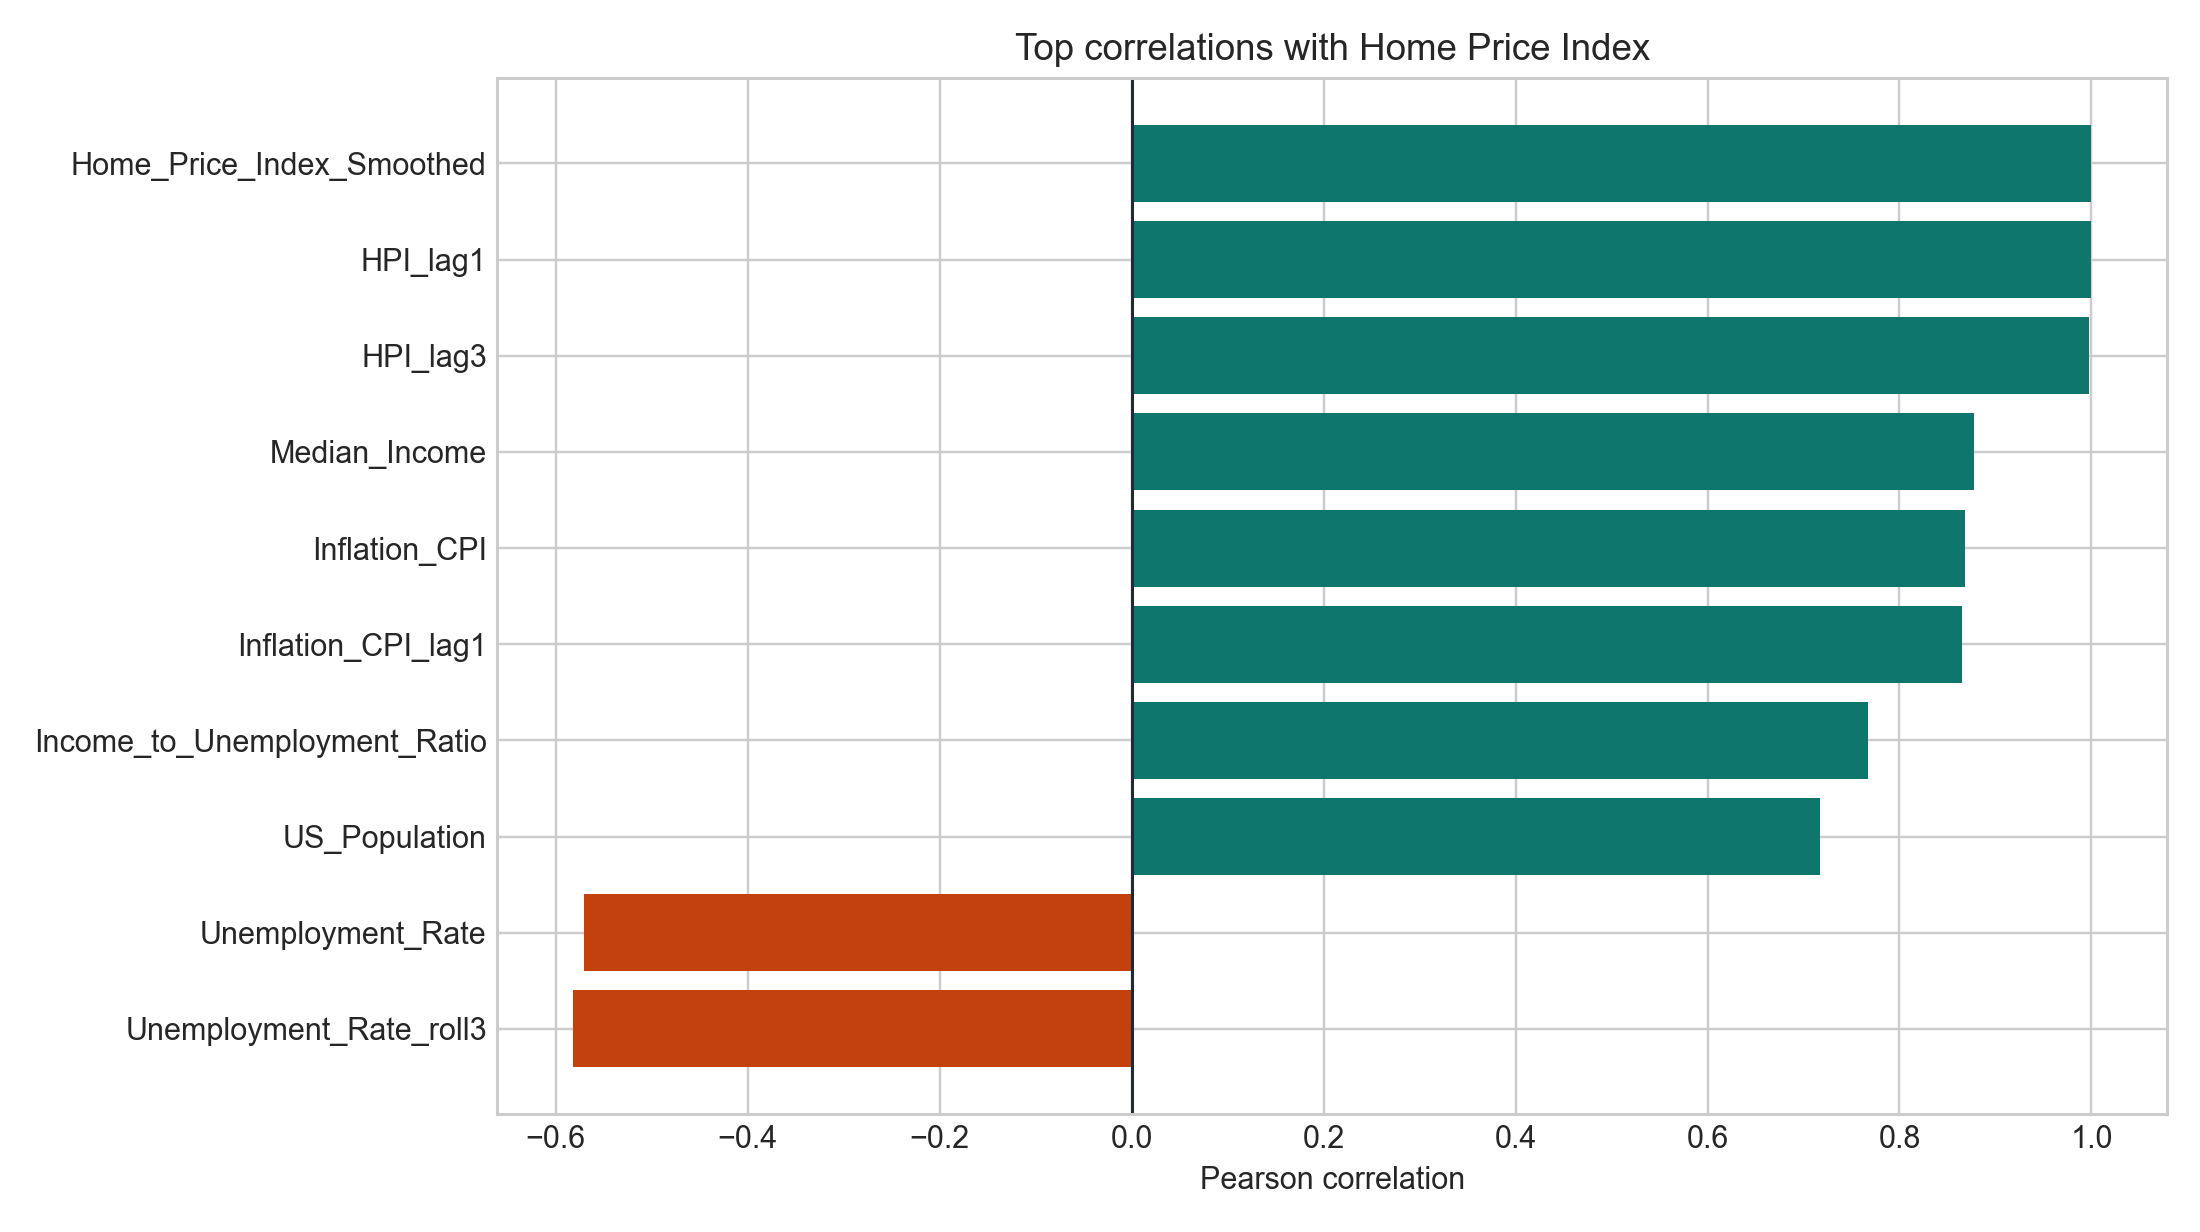
\includegraphics[width=0.92\textwidth]{figures/correlation_results.png}
\caption{Strongest correlations with the Home Price Index in the project dataset.}
\label{fig:generated_corr}
\end{figure}

The strongest linear relationships with the target are: \texttt{Home\_Price\_Index\_Smoothed} (1.00), \texttt{HPI\_lag1} (1.00), \texttt{HPI\_lag3} (1.00), \texttt{Median\_Income} (0.88). These correlations support the paper-review conclusion that housing prices should be interpreted through several linked economic forces, not through a single variable.

\begin{table}[H]
\centering
\begin{tabular}{lrrrr}
\toprule
\textbf{Model} & \textbf{MAE} & \textbf{RMSE} & \textbf{$R^2$} & \textbf{CV $R^2$} \\
\midrule
Linear Regression & 0.661 & 0.797 & 0.999 & 0.994 \\
Ridge Regression & 3.715 & 4.162 & 0.984 & -3.135 \\
Gradient Boosting & 65.816 & 73.669 & -4.148 & -2.458 \\
Decision Tree & 66.218 & 73.750 & -4.159 & -3.315 \\
Random Forest & 69.077 & 76.105 & -4.494 & -2.619 \\
KNN & 74.459 & 79.883 & -5.053 & -4.314 \\
SVR & 103.767 & 109.606 & -10.395 & -7.678 \\
\bottomrule
\end{tabular}
\caption{Generated regression comparison on the chronological test set.}
\label{tab:generated_model_metrics}
\end{table}

The best test-set model in this generated run is \textbf{Linear Regression}, with \(R^2=0.999\), RMSE \(=0.797\), and MAE \(=0.661\). Because the dataset includes lagged and smoothed price features, the linear model can extrapolate the rising trend very effectively. The weaker tree-model scores are also informative: tree ensembles can capture non-linear interactions, but they may struggle when the test period moves beyond the range learned during training.

\begin{figure}[H]
\centering
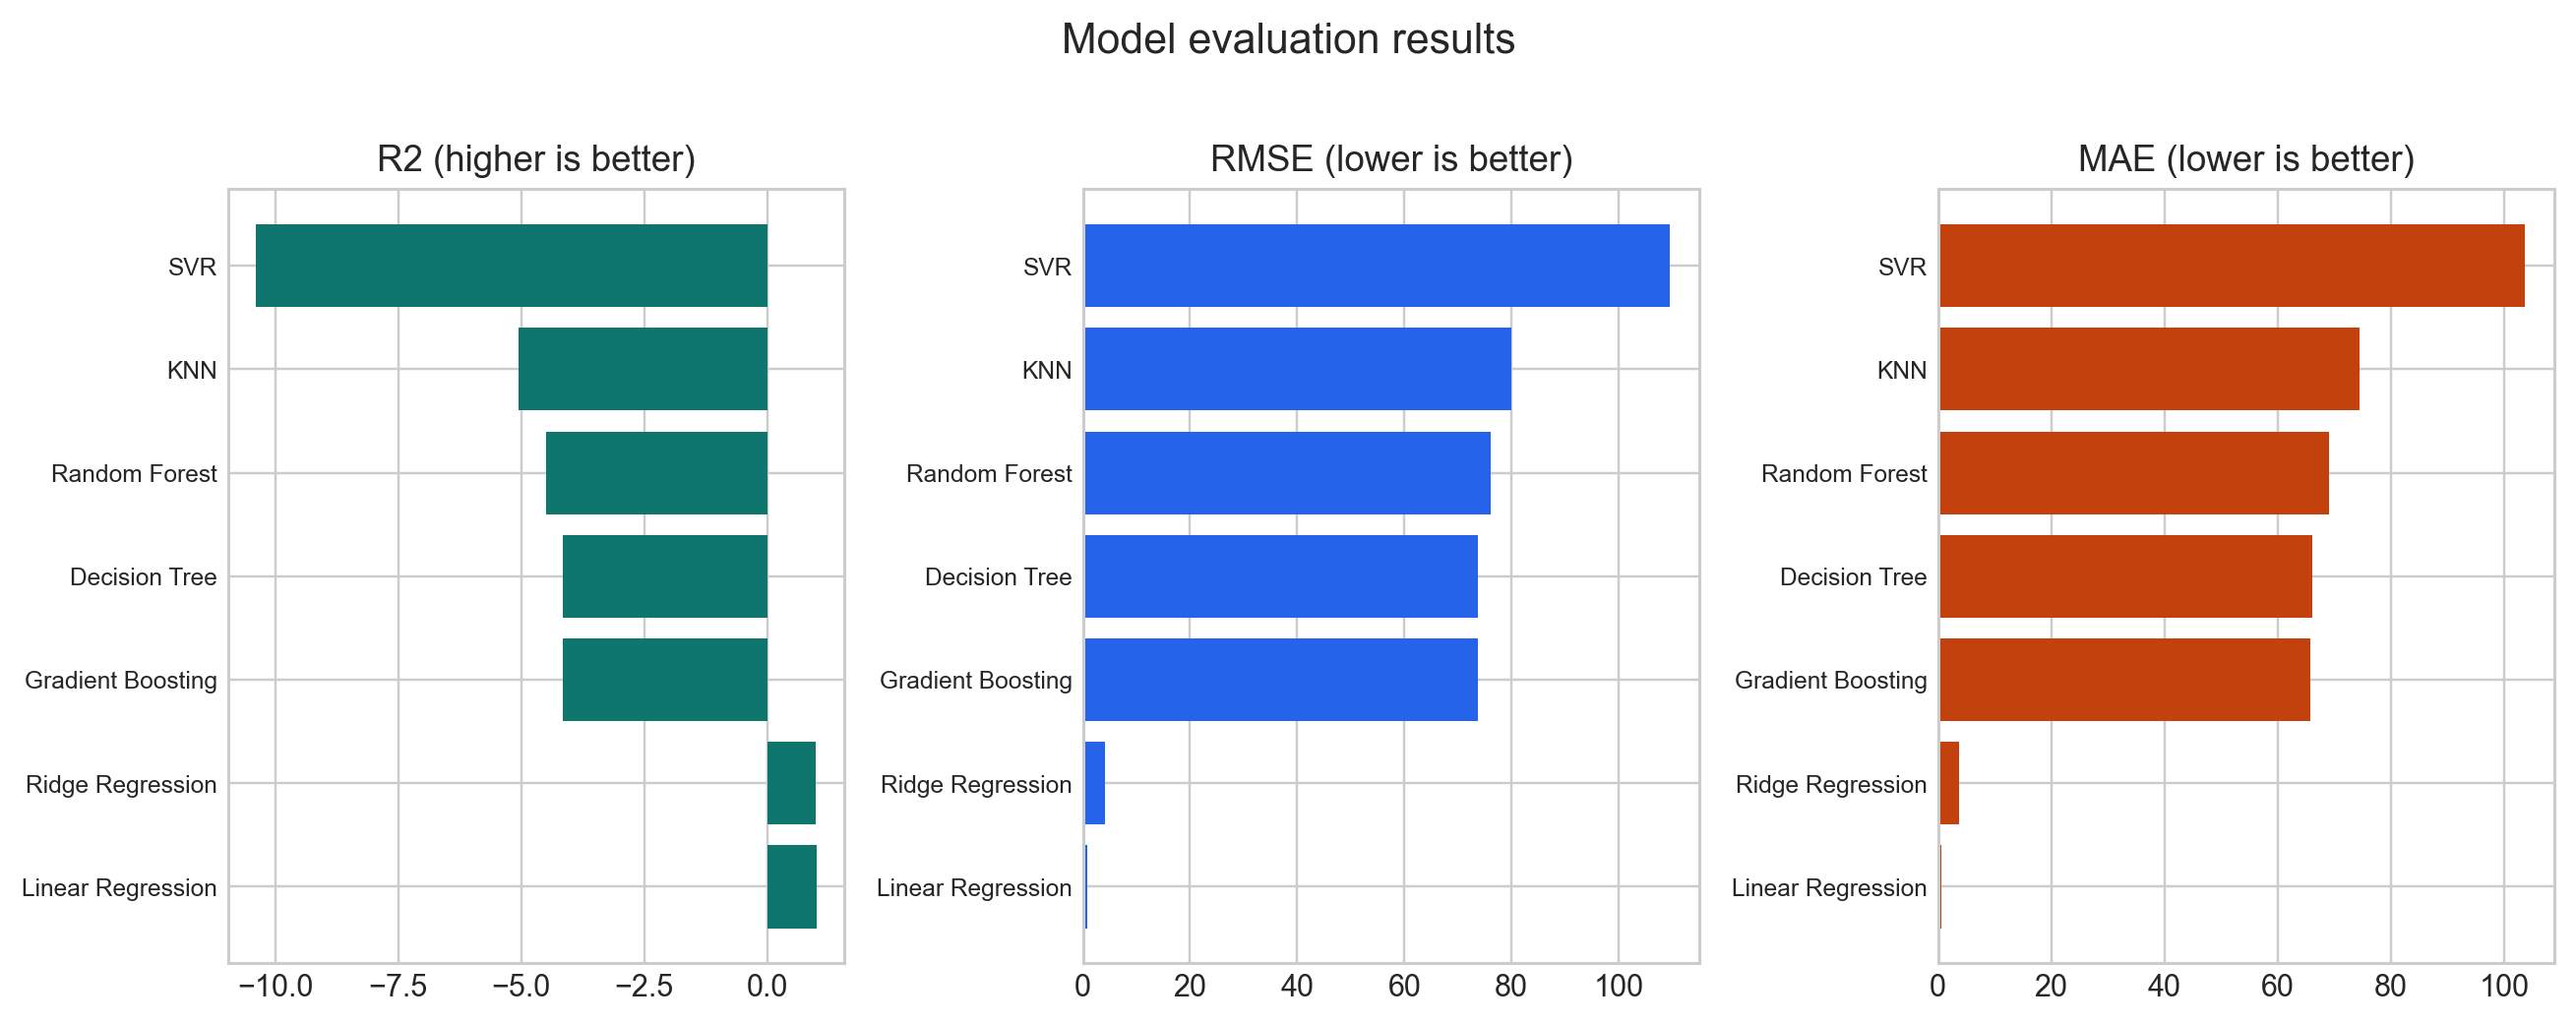
\includegraphics[width=0.98\textwidth]{figures/model_evaluation_results.png}
\caption{Evaluation graphics generated from the model comparison module.}
\label{fig:generated_eval}
\end{figure}

\begin{figure}[H]
\centering
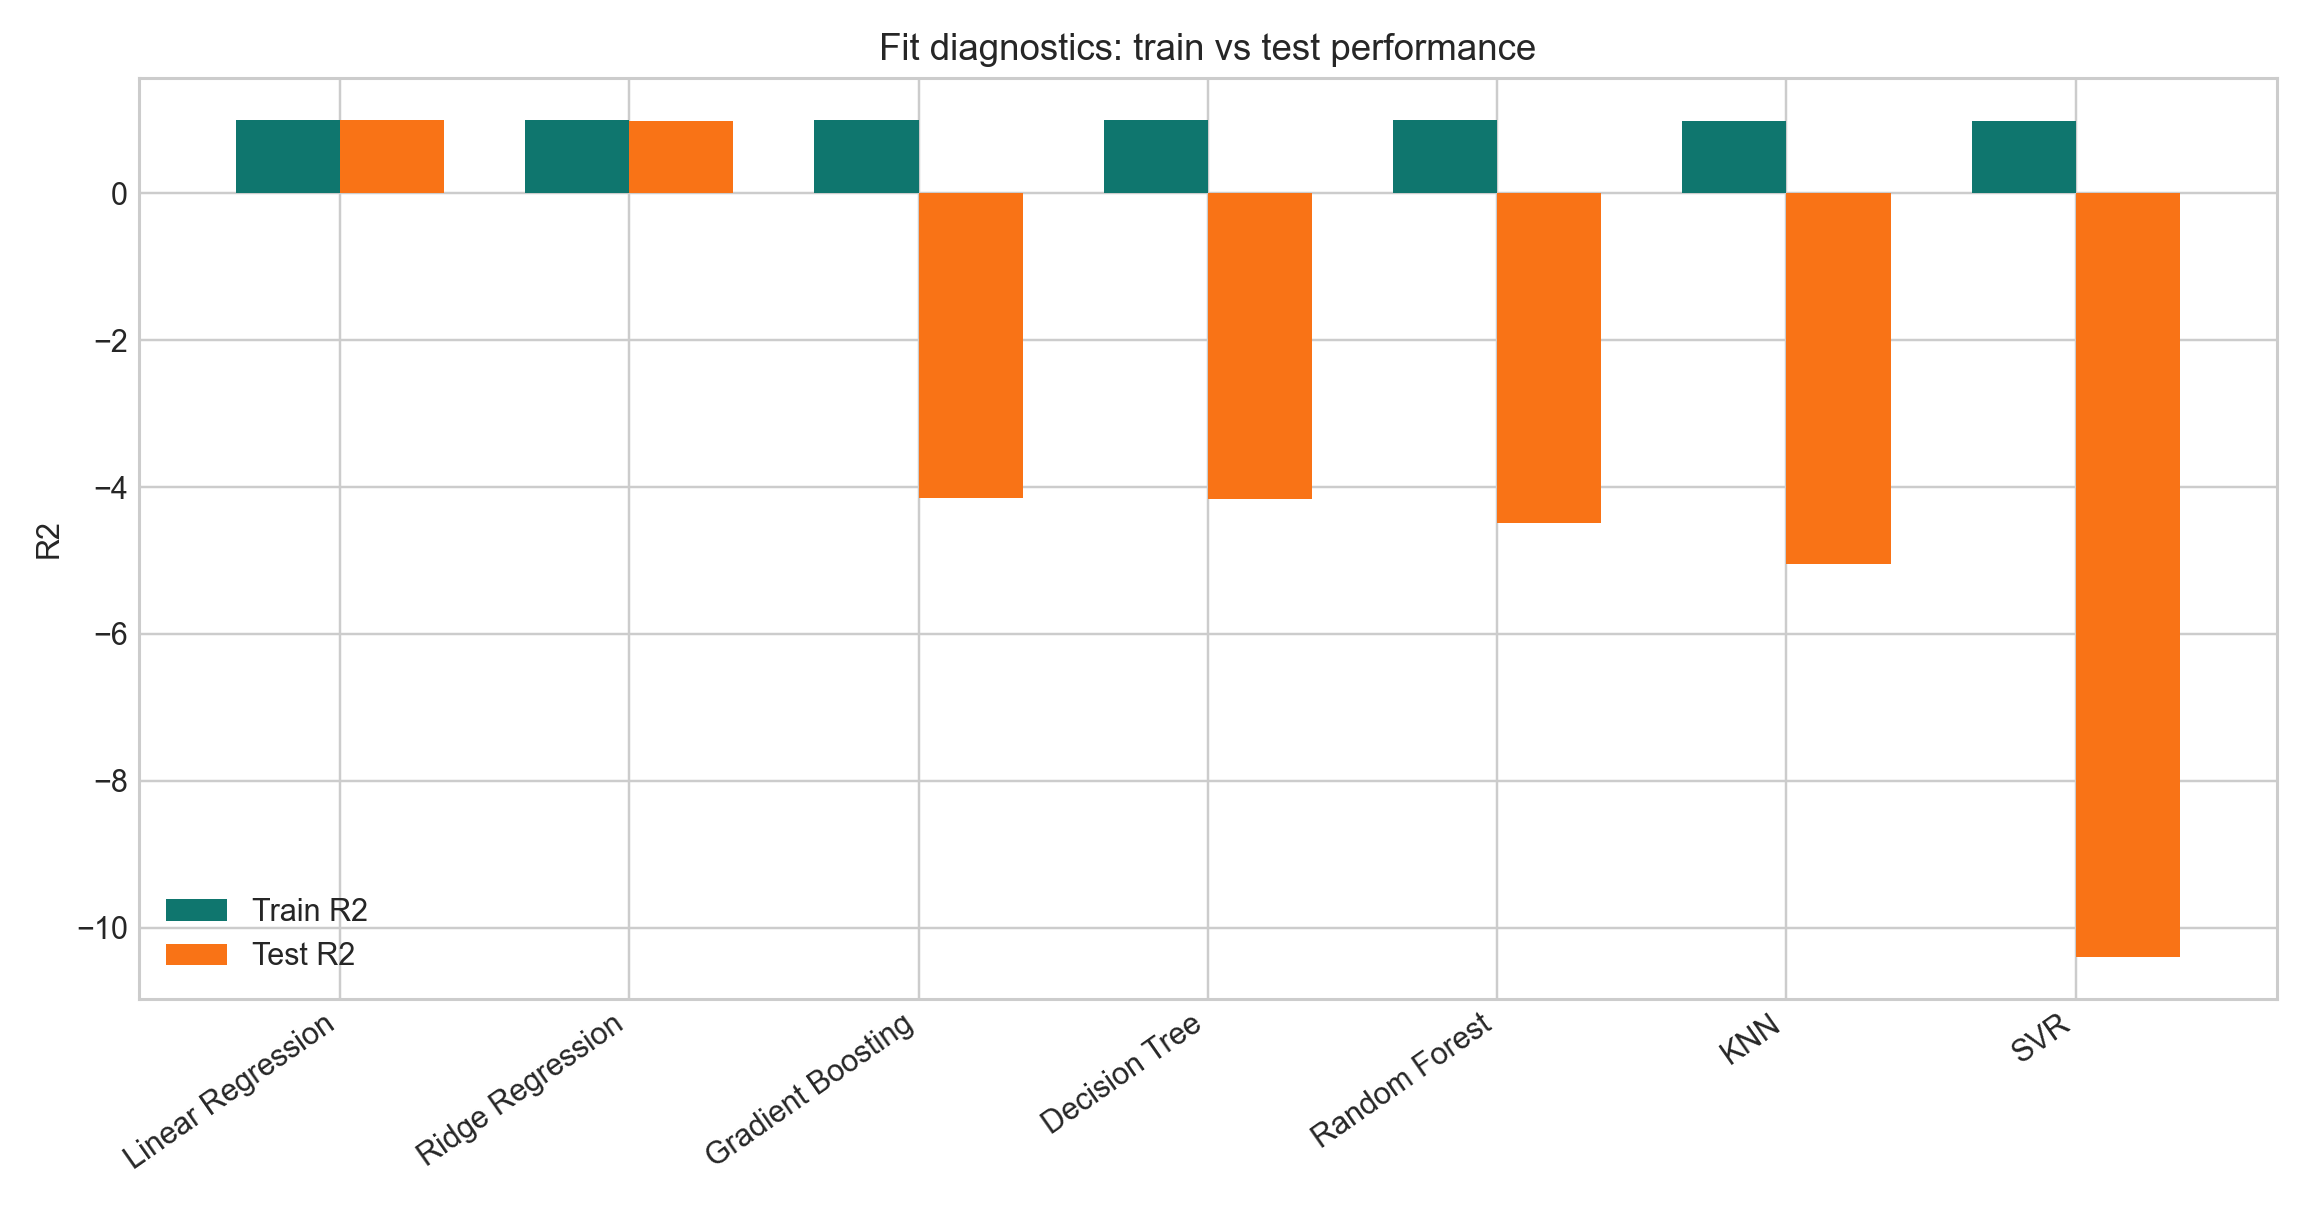
\includegraphics[width=0.92\textwidth]{figures/fit_diagnostics_results.png}
\caption{Fit diagnostics comparing train and test performance.}
\label{fig:generated_diag}
\end{figure}

The diagnostics figure shows whether a model generalizes beyond the training period. A large train-test gap indicates overfitting risk, while a weak score on both sets indicates underfitting. This is why the final project does not rely only on the highest raw score: it also asks whether the result is stable and explainable.

\begin{figure}[H]
\centering
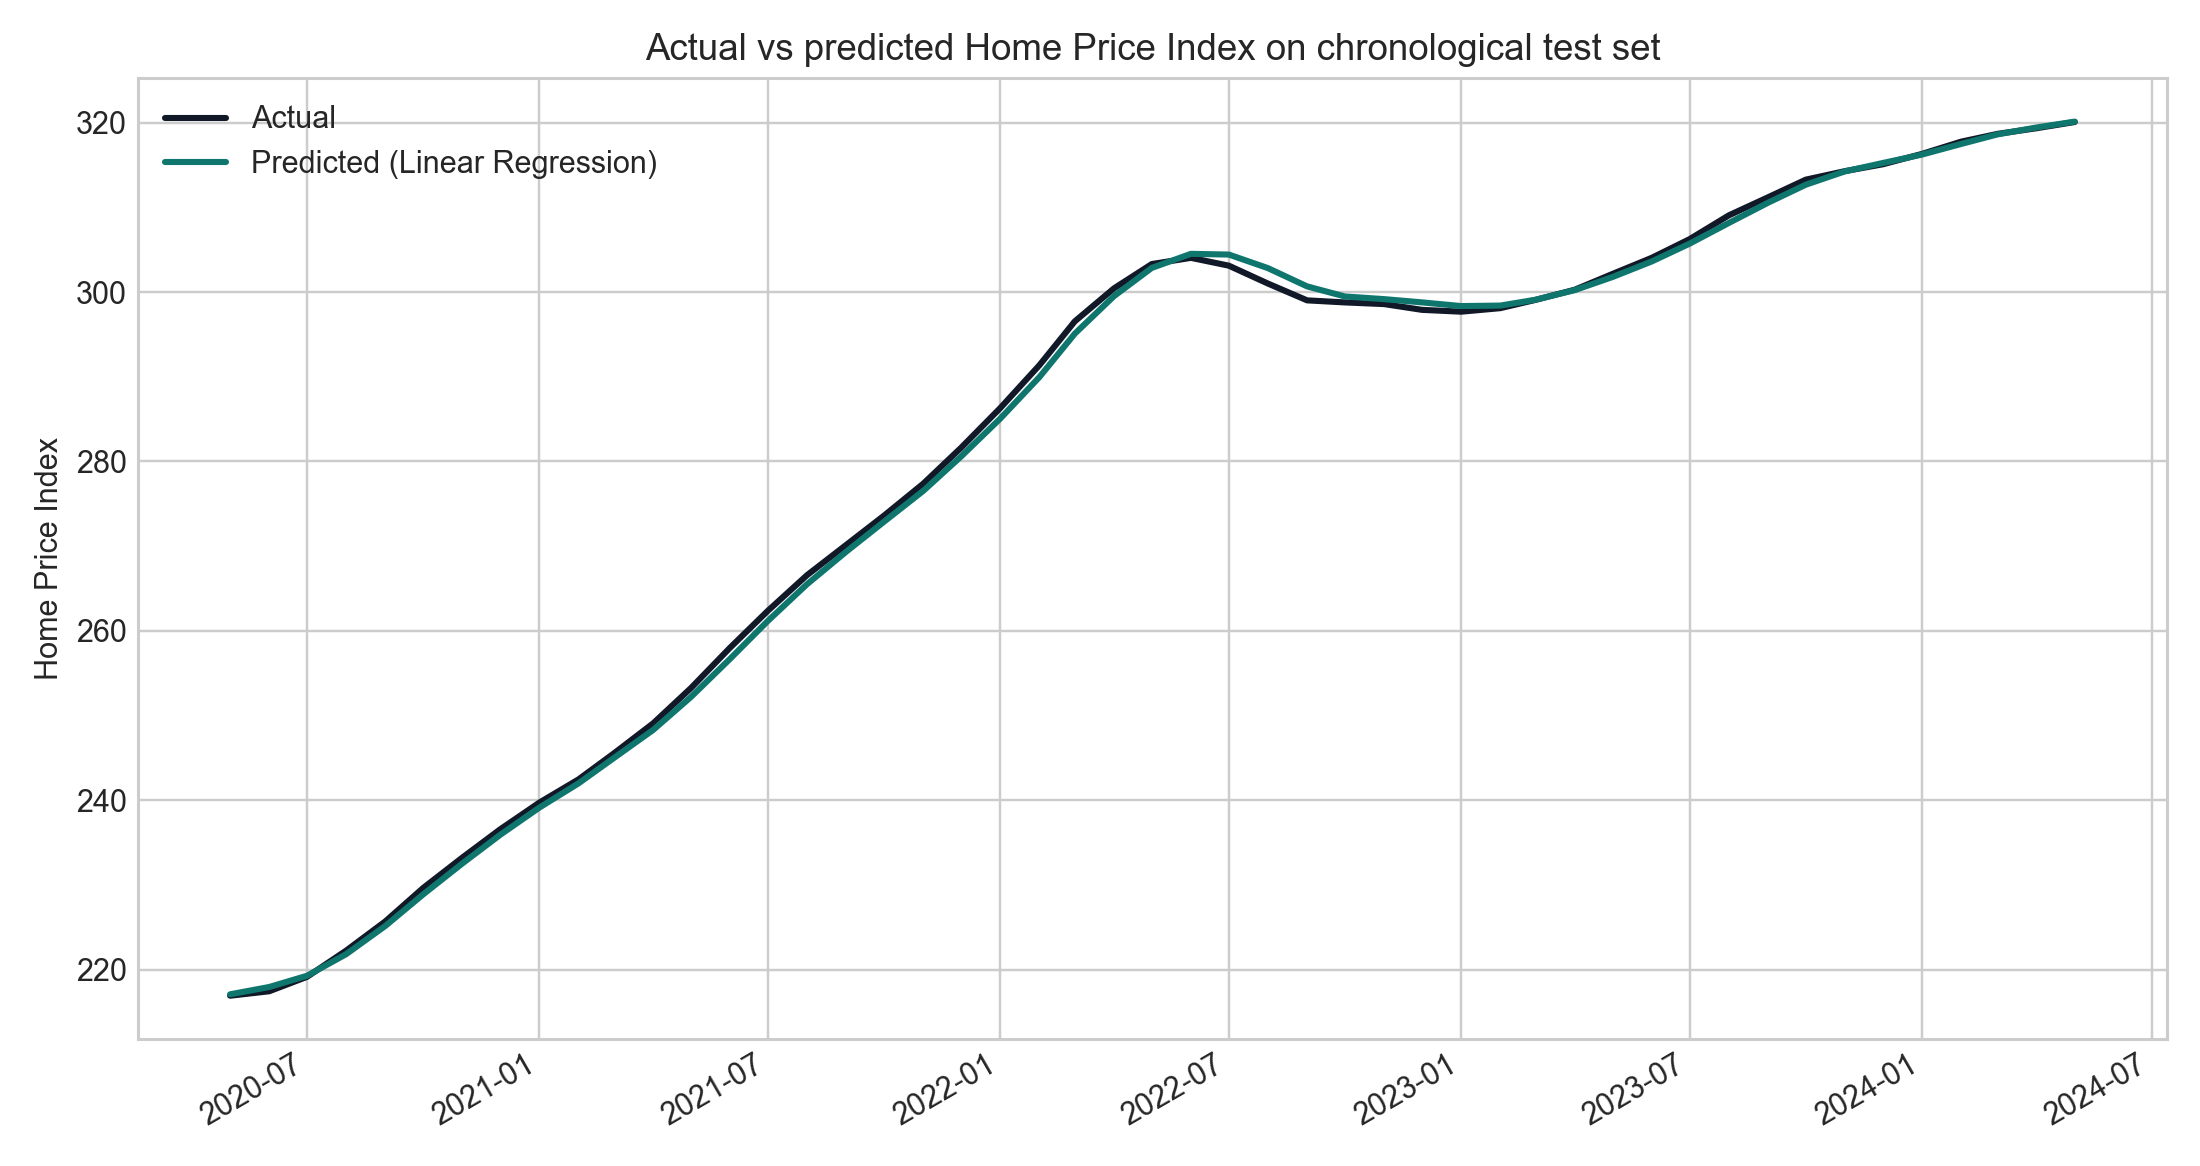
\includegraphics[width=0.92\textwidth]{figures/actual_vs_predicted_results.png}
\caption{Actual and predicted Home Price Index for the best model on the test period.}
\label{fig:generated_pred}
\end{figure}

\begin{figure}[H]
\centering
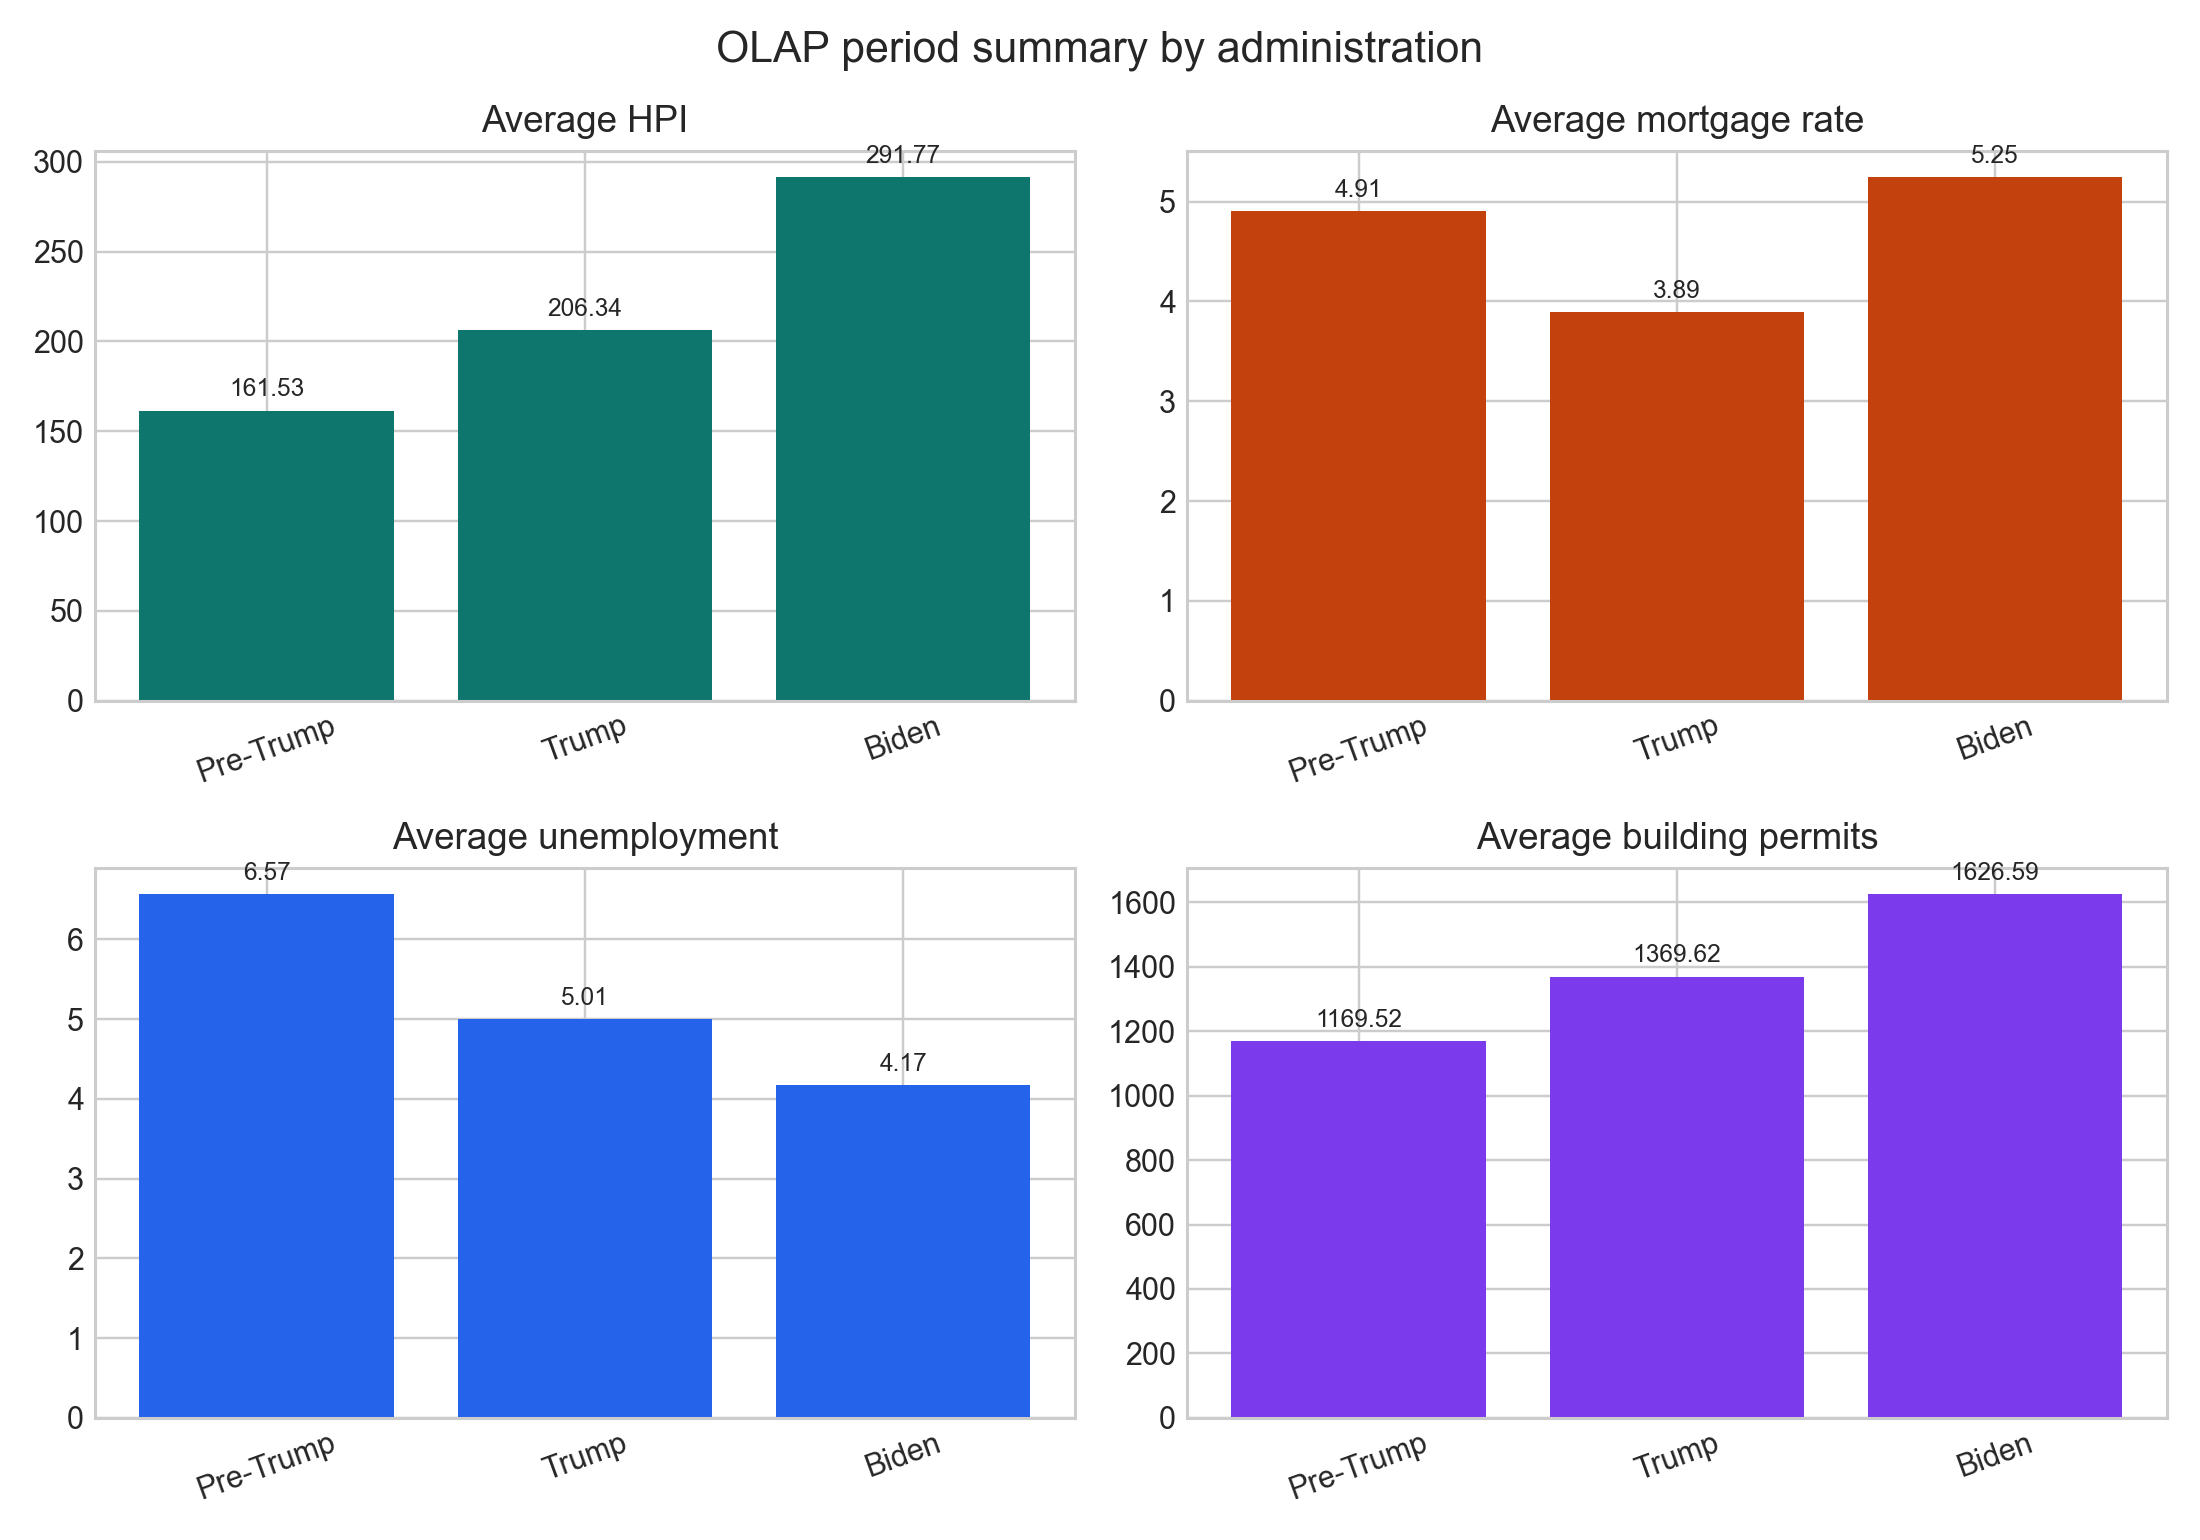
\includegraphics[width=0.95\textwidth]{figures/olap_period_results.png}
\caption{OLAP-style period comparison by administration.}
\label{fig:generated_olap}
\end{figure}

The OLAP summary shows that the highest average Home Price Index appears during the \textbf{Biden} period, while the highest average mortgage-rate pressure appears during the \textbf{Biden} period. This result is useful for the paper-review argument: prices and affordability pressure can rise together when supply, timing, and market inertia slow the response of prices.
